\documentclass[runningheads,a4paper]{llncs}

\usepackage{amssymb}
\setcounter{tocdepth}{3}
\usepackage{graphicx}
\usepackage{amsmath}
\usepackage{verbatim}
\usepackage[margin=0.9in]{geometry}
%\usepackage{amsfonts}
%\usepackage{amsthm}
\usepackage{subfigure}
\usepackage{mathtools}
%\usepackage{caption}
%\usepackage{subcaption}
%\usepackage{cite}
\usepackage{hyperref}
\usepackage{url}
\urlstyle{same}
\newcommand{\keywords}[1]{\par\addvspace\baselineskip
\noindent\keywordname\enspace\ignorespaces#1}

\makeatletter
\let\c@lemma=\c@theorem
\let\c@corollary=\c@theorem
\let\c@fact=\c@theorem
\makeatother

\let\realendproof=\endproof
\def\endproof{\hspace*{\fill}$\Box$\realendproof}


\begin{document}

\title{Poker Chips, Earthquakes, and Computation}
\titlerunning{Poker Chips, Earthquakes, and Computation}

\author{Perry Kleinhenz \and Fermi Ma \and Erik Waingarten}
%
\authorrunning{Perry Kleinhenz \and Fermi Ma \and Erik Waingarten}
% (feature abused for this document to repeat the title also on left hand pages)

% the affiliations are given next; don't give your e-mail address
% unless you accept that it will be published
\institute{
\protect\url{{pkleinhe, fermima,eaw}@mit.edu}}

\maketitle

\section{Introduction}

\emph{Written by Fermi Ma, edited by Erik Waingarten and Perry Kleinhenz.}\\

\noindent In this paper, we investigate the following problem:

\vbox{
\noindent
\begin{quote}
Each node of an infinite grid graph contains some nonnegative number of chips. An earthquake hits one node that has at least four chips and redistributes them so that one chip moves to each of its four neighbors.
\end{quote}
}

In Section~\ref{Definitions and Notation}, we formalize the terminology and operations we use to analyze the problem. In particular, we formalize the effects of earthquakes, as well as what it means for a board of chips to be finite or infinite. 
In Section~\ref{Stability of Finite Boards}, we introduce a spread function that maps finite board configurations to positive integers. 
We then use the fact that earthquakes strictly increase the value of this spread function to show that finite boards cannot cycle back to previous configurations. We also show that the number of possible configurations a finite board can be transformed into by earthquakes is bounded. These two results together will show that all finite boards reach a steady state. 
In Section~\ref{Order of Redistribution}, we show that for a given board the number of times a particular square must be hit by an earthquake in order for a board to stabilize is independent of the order in which the earthquakes occur. 

For the remainder of the paper, we consider other approaches and extensions of the problem. 
%In  Section~\ref{Time until Stability}, we present results from our computer simulations of repeated earthquakes. In particular, we look at the starting arrangement where all of the board's $n$ chips are initially on one central square.
%We conjecture based on experimental evidence that such arrangements stabilize after $\Theta(n \log n)$ global earthquakes. 
In Section~\ref{Board Variants: d-Trees}, we generalize away from the infinite grid graph and consider what happens when a similar process happens on tree graphs of infinite size. 
Finally, in Section~\ref{Computing with Chips} we present a model of computation based on the poker chip board and show how to construct simple Boolean circuits.
\section{Definitions and Notation}
\label{Definitions and Notation}

\emph{Written by Erik Waingarten, edited by Fermi Ma and Perry Kleinhenz.}\\

First, we formalize the definition of a board. The board is an infinite grid graph with a nonnegative number of chips placed at each node
\begin{figure}
\begin{center}
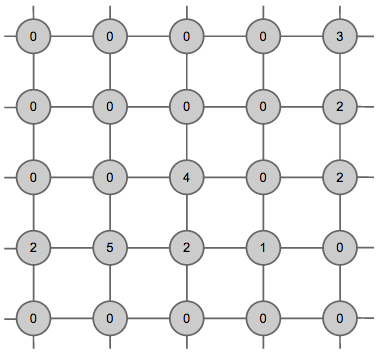
\includegraphics[scale=0.5]{grid1.png}
\end{center}
\caption{A finite component of the grid}
\end{figure}

\begin{figure}
\label{cartesiangrid}
\begin{center}
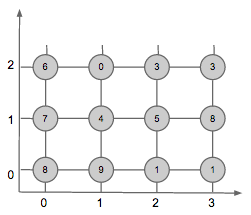
\includegraphics[scale=0.8]{cartesiangrid.png}
\end{center}
\caption{A finite component of the grid with coordinates}
\end{figure}

We can coordinatize the grid graph by labeling it like the standard Cartesian grid, where we fix one node to be the origin $(0,0)$, and we index all other nodes by integer coordinates $(i,j)$. We will define the board as a function from the Cartesian grid to the nonnegative integers.

\begin{definition} Boards are functions $b$ from $\mathbb{Z}^2 \to \mathbb{Z}_{\geq 0}$.
\end{definition}

This function maps node labels given as integer coordinates to chip stack sizes. For example, in Figure \ref{cartesiangrid} the board $b$ has 8 chips at the node with coordinate $(3,1)$, so we write $b(3,1) = 8$.

\begin{definition} Let $n(i,j)$ be the set of neighbors of node $(i,j)$
\begin{equation*}
n(i,j) = \{ (i+1, j), (i-1, j), (i, j-1), (i, j+1) \}.
\end{equation*}
\end{definition}

We now formally define the earthquake operation. Recall that an earthquake hits a node that has 4 or more chips and moves 1 chip to each of the node's 4 neighbors. 

\begin{definition}
Let $E_sb$ be the board that results from an earthquake hitting board $b$ at node $s$. If $b(s) \geq 4$, then
\begin{align*}
E_sb(s) &= b(s)-4,\\
E_sb(t) &= b(t)+1 \hspace{.5cm} \forall t \in n(s).\\
\end{align*}
if $b(s) < 4$, the earthquake has no effect and $E_sb = b$. 
\end{definition}

\begin{figure}
\centering
\subfigure[Board before earthquake.]{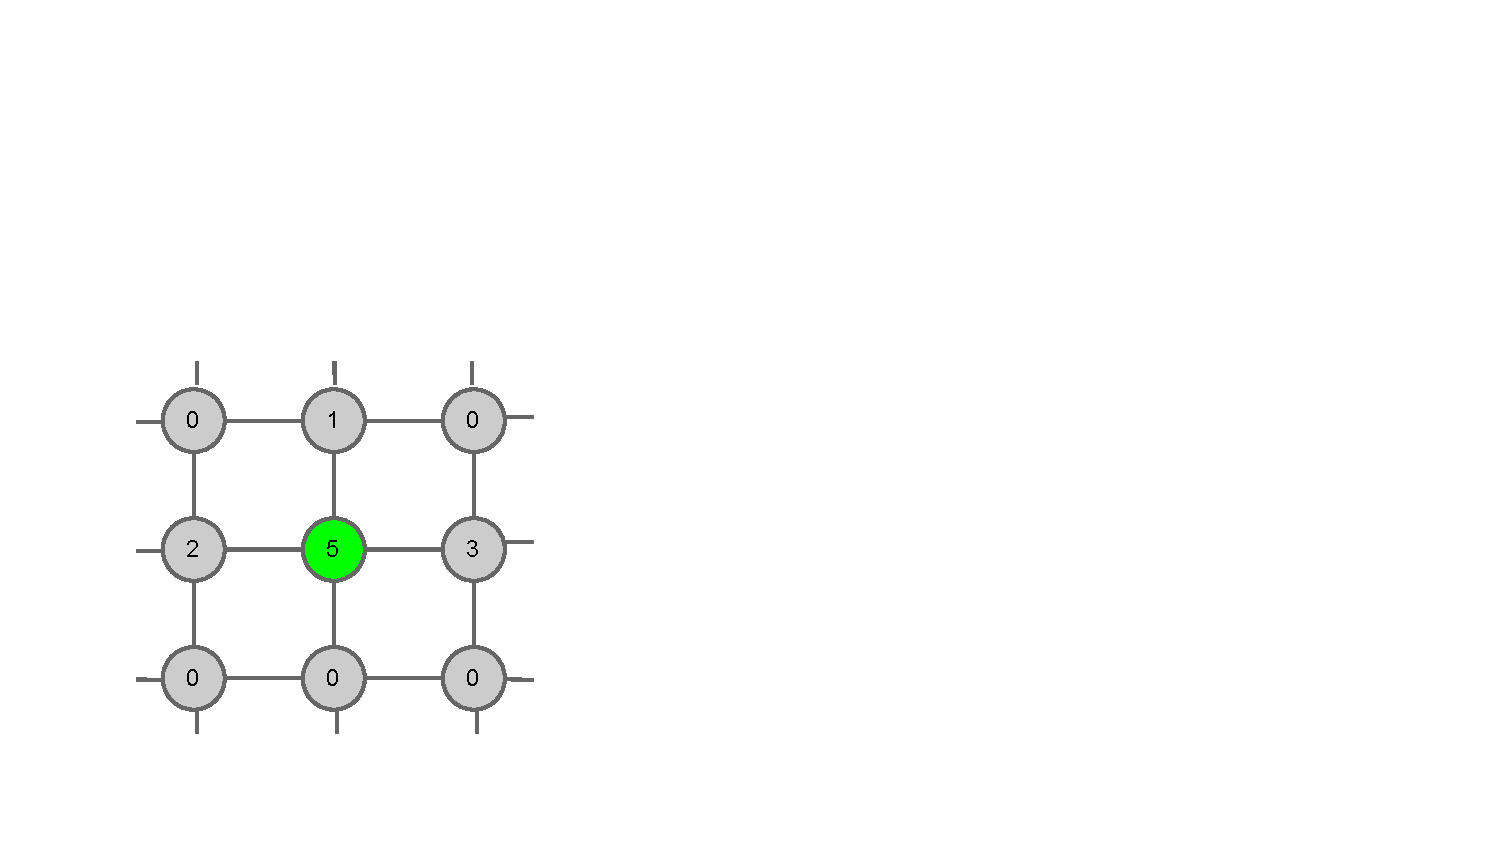
\includegraphics[width=0.25\linewidth]{action1.pdf}\label{fig:boardbeforeearthquake}}
\qquad\qquad
\subfigure[Board after earthquake to active square]{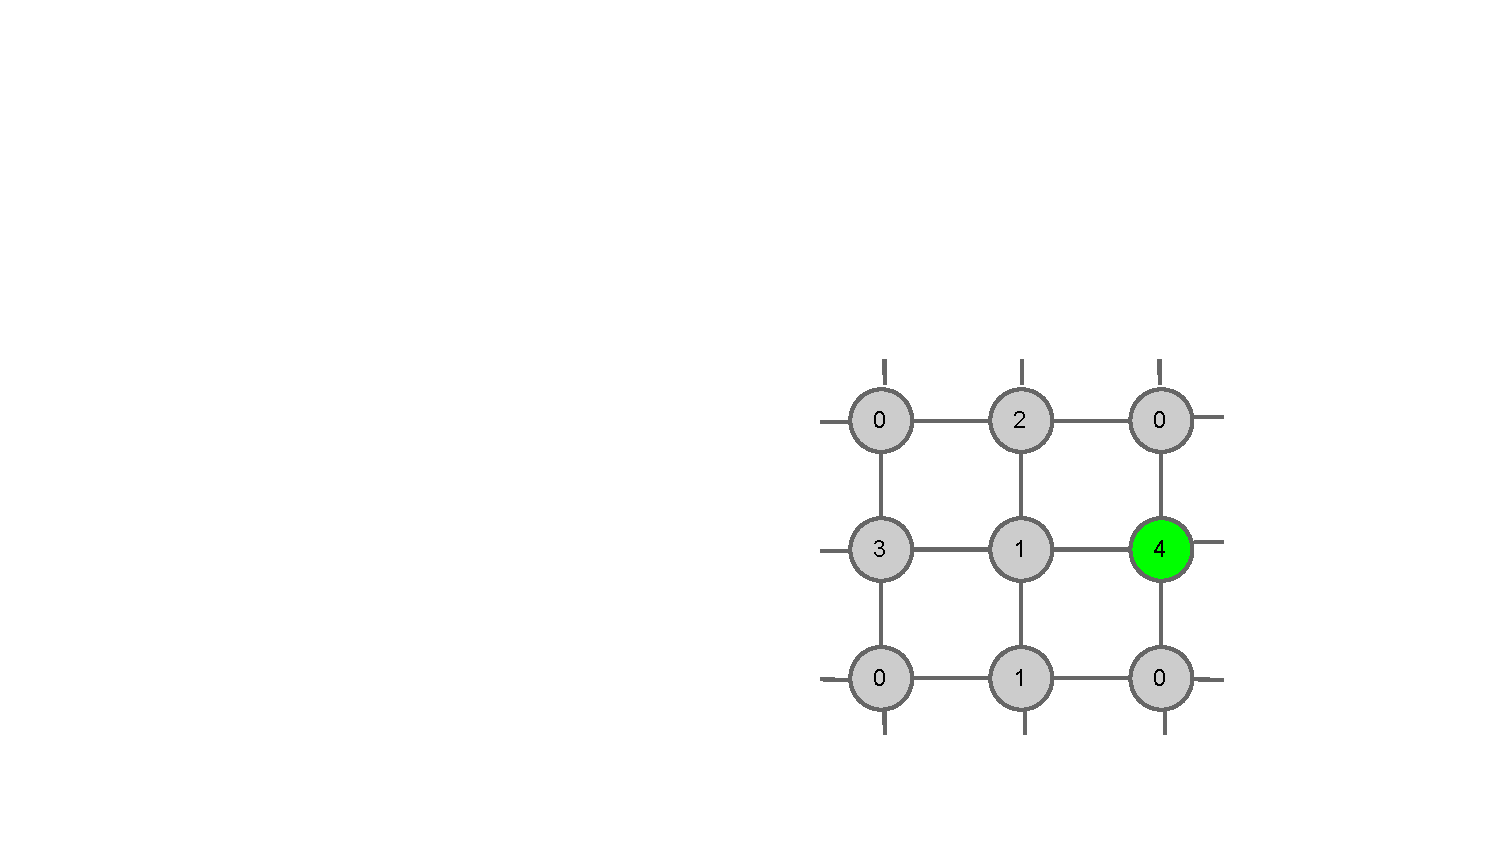
\includegraphics[width=0.25\linewidth]{action2.pdf}\label{fig:boardafterequarthquake}}
\caption{Earthquake applied to board. Green signifies nodes with more than 4 chips}
\label{fig:earthquakeexample}
\end{figure}

Generally, when we refer to an earthquake, we restrict our attention to earthquakes that actually change the state of the board. 

Often, a number of earthquakes will hit a board $b$. We represent the result of multiple earthquakes by a composition of the earthquake functions. For example, if an earthquake hits node 1, then node 2, and finally node 3, the resulting board is written as $E_3E_2E_1b$.

Now that we have formalized the earthquake operator, we make precise the definition of stability.
\begin{definition}
A board is stable if all nodes contain values strictly less than 4. 
\end{definition}
This definition corresponds with the intuitive notion of a process that has stabilized, as stable boards can no longer be changed by earthquake operations.

We also formalize the notion of $\emph{finite}$ and $\emph{infinite}$ boards, a distinction we will refer to extensively throughout this paper.

\begin{definition} 
A board is finite if the total number of chips on it is finite. Otherwise we say a board is infinite. 
\end{definition}

Finally, we use the above definitions to define global earthquakes, which will be defined only for finite boards. 
\begin{definition}
Given a finite board $b$, a global earthquake is given by applying one earthquake to every square in $b$ that initially has 4 or more chips.
\end{definition}

We will see in Section~\ref{Order of Redistribution} that the order in which earthquakes are applied does not matter, and thus global earthquakes are well-defined without the need for an ordering on the individual earthquakes. In order to avoid the case where there may be infinitely many squares with 4 or more chips, we only define global earthquakes for finite boards.

\section{Stability of Finite Boards}
\label{Stability of Finite Boards}
\emph{Written by Erik Waingarten, Edited by Fermi Ma and Perry Kleinhenz.}

In this section, we show that any finite board will become stable after a finite number of earthquakes. We first introduce a spread function that maps boards to the positive integers. We demonstrate that the spread function strictly increases after earthquakes are applied, which will imply that an earthquake irreversably changes a board configuration. In other words, we can never return to a given board arrangement.

We then give a bound on the maximum number of board configurations a finite board can be transformed into by earthquakes. We will argue that since a finite number of boards are reachable and board states are never revisited, eventually this process must terminate. Thus, we eventually reach a stable board where no earthquakes will change the board.

To define the spread function, we fix one coordinate on a board $b$ as the origin $(0,0)$, and we define the \emph{taxicab distance} $d(s)$ of a node $s$ on the board to be $|s_x| + |s_y|$, where $s_x$ is the $x$ coordinate of node $s$, and $s_y$ is the $y$ coordinate of node $s$. Then the spread function is
\begin{equation*}
\Psi(b) = \sum_{\text{all nodes }s}b(s)d(s)^2.
\end{equation*}

Essentially the function sums up the number of chips on a given node weighted by the taxicab distance to the origin squared. The motivation for this definition is that the spread function gives a measure of how ``spread out" the chips on a board are. Intuitively, earthquakes takes chips that are condensed in a single pile and spreads them out over a greater area. We capture this in the following lemma:

\begin{lemma}
\label{spreadfunction}
Suppose an earthquake hits node $s$ of a finite board $b$, producing the board $E_sb \neq b$. Then
\begin{equation*}
\Psi(E_sb) > \Psi(b),
\end{equation*}
so the earthquake strictly increases the spread of the board.
\end{lemma}
\begin{proof}
The chip stacks of the two boards are the same at all nodes except at $s$ and $n(s)$, the nodes that neighbor $s$. Thus, the contribution to $\Psi$ is the same at all nodes except for those 5.

Let the taxicab distance to $s$ be $d_s$. Then the contribution to the spread function from node $s$ decreases from $b(s)d_s^2$ to $(b(s)-4)d_s^2$.

Out of the 4 nodes in $n(s)$, some have a taxicab distance of $d_s+1$, and the rest are at distance $d_s-1$. In particular, if $s$ is not exactly on the $x$ or $y$ axis, exactly 2 neighboring nodes are at $d_s+1$, and exactly 2 are at distance $d_s-1$. If $s$ is on either the $x$ or $y$ axis, then 3 nodes are at distance $d_s+1$, and 1 neighboring node is at distance $d_s-1$. We only need a lower bound for the increase in the spread function, so we focus only on the case where exactly 2 neighboring nodes are at distance $d_s+1$, as it can be shown that this case leads to a strictly smaller increase than the other.

Suppose that the two neighboring nodes at distance $d_s+1$ have chip stacks of $n_1$ and $n_2$ originally. Then their contribution to the spread function goes from $n_1(d_s+1)^2$ and $n_2(d_s+1)^2$ to $(n_1+1)(d_s+1)^2$ and $(n_2+1)(d_s+1)^2$. If the other two nodes at distance $d_s-1$ have chip stacks of $n_3$ and $n_4$, their contribution to the spread function goes from $n_3(d_s-1)^2$ and $n_4(d_s-1)^2$ to $(n_3+1)(d_s-1)^2$ and $(n_4+1)(d_s-1)^2$.

Omitting the algebraic details, we find that summing up the changes in the spread function gives
\begin{equation*}
 \Psi(E_sb) - \Psi(b) = 4,
 \end{equation*}
which completes the proof.
\end{proof}

\begin{corollary}
\label{norepeats}
A finite board can never return to a previous state via a sequence of earthquakes.
\end{corollary}
\begin{proof}
Suppose for the sake of contradiction that this is possible, and that $b = E_1E_2\cdots E_kb$ for some sequence of earthquakes $E_1,E_2,\dots,E_k$. Lemma~\ref{spreadfunction} shows that $\Psi(b) < \Psi(E_1E_2\cdots E_kb)$, which is a contradiction.
\end{proof} 

Now that we have shown that an earthquake can never transform a finite board into a board it was previously we will give a bound on the number of different boards that earthquakes can transform a given finite board into.
\begin{lemma}
\label{finiteextension}
Suppose there are a total of $C$ chips on the board, and $b$ is nonzero in the region $[i_{min}, i_{max}] \times [j_{min}, j_{max}]$ (equivalently, all chips on the board are in this region). Then after any sequence of earthquakes, the resultant board is nonzero only in the region $[i_{min}-C, i_{max}+C] \times [j_{min}-C, j_{max}+C]$ .
\end{lemma}

\begin{proof}
This follows from the observation that if a row / column of the board contains at least one chip, it will always contain at least one chip. Note that this follows from the fact that an earthquake operation can never cause a board to break this property; if a row / column is affected by an earthquake operation, at least 2 chips stay inside that row / column.

Now consider the maximum value $x$ coordinate of the board that chips can ever ``reach". An earthquake must first move a chip to the column given by $x$ coordinate $i_{max} +1$, and a chip will always stay there. The same argument follows for $i_{max} + 2$, and so on, but we can only do this up until $i_{max} +C$. The same argument works in any direction, so we can never leave the region $[i_{min}-C, i_{max}+C] \times [j_{min}-C, j_{max}+C]$.
\end{proof}

We are now ready to show that all finite boards will reach a stable state. 

\begin{theorem} If $b$ is a finite board that is repeatedly hit by earthquakes, it must eventually reach a stable state. 
\end{theorem}
\label{finitestability}
\begin{proof}
Lemma~\ref{finiteextension} implies that a finite board with $C$ total chips can only ever occupy a finite number $D$ of squares. This implies a finite upper bound of $\binom{D+C-1}{D-1}$ possible boards (via an elementary combinatorics argument of how to distribute $C$ identical objects among $D$ distinguishable slots).

In addition, Corollary~\ref{norepeats} tells us that we never visit a board state more than once. Thus, since we have a finite number of reachable board states, and a nontrivial earthquake operation always outputs a previously unvisited board, a sequence of earthquake operations must eventually end. At this end state, the board cannot allow further nontrivial earthquakes, and is stable by definition.
\end{proof}

We can use our result for finite boards to show that earthquakes will never cause infinite boards to revisit a prior arrangement.  

\begin{corollary}
Suppose $b$ is an infinite board. If $E_s b \neq b$, then no application of earthquakes to $E_s b$ can produce $b$.
\end{corollary}

\begin{proof}
We will proceed by contradiction. Assume otherwise, so there exists some sequence $\{s_1, s_2, \ldots, s_k\}$ such that after applying an earthquake to each of these locations on $E_s b$ the resultant board is $b$.
However, we can bound the size of the locations affected by $\{s, s_1, s_2, \ldots, s_k \}$, call it $R$.  This infinite board behaves the same way as a finite board with the same values on $R$ and 0 outside of $R$. But this means that earthquakes transformed a finite board back into a previous state which contradicts Lemma ~\ref{finiteextension}. Therefore infinite boards cannot be transformed back into a previous state.
\end{proof}

\section{Order of Redistribution}
\label{Order of Redistribution}

\emph{written by Fermi Ma and Perry Kleinhenz, edited by Erik Waingarten.}\\

Now that we have shown that all finite boards will eventually reach a stable state we would like to know if the order in which these earthquakes occur matters. More specifically, if we consider some finite starting board and two sequences of earthquakes that stabilize the board, we would like to know if the resultant board is the same for both sequences. 

In fact we are able to show that not only is this final board the same but that the number of earthquakes that target a particular node in order to stabilize the board is invariant of the order in which the earthquakes occur. We show this by first describing conditions under which we can rearrange a sequence of earthquakes without changing the resultant board. We then define a process that rearranges a sequence of earthquakes without changing the final board state and for a given board will always produce the same sequence.\\

First, we formalize the notion of earthquakes that are ``allowed to happen".

\begin{definition}
We say that an earthquake $E$ is valid if the node it targets has at least $4$ chips on it. 
We say that a sequence of earthquakes $E_1, E_2, \ldots E_n$ is a valid sequence of earthquakes if each earthquake is valid when applied one after another. 
\end{definition}


For ease of notation we also introduce an indicator function
\begin{definition}
We define the indicator function $[[\cdot]]$ as 
\begin{equation*}
[[A]] = \begin{cases} 1 \text{ if A is true} \\ 0 \text{ if A is false} \end{cases}.
\end{equation*}
\end{definition}

Recalling that $n(s)$ refers to the set of neighbors of the square $s$ we note that if an earthquake $E$ is valid then we can write it in terms of this indicator function.
\begin{lemma} 
\label{earthquakeredefine}
Consider a board $b$. If $E$ is a valid earthquake, then 
\begin{equation*}
E_s b(x) = b(x) + 1[[ x \in n(s)]] - 4[[x =s]].
\end{equation*}
\end{lemma}
\begin{proof}
This follows directly from the definition of an earthquake and a valid earthquake. 
\end{proof}

Now we can show that switching the order of two earthquakes with certain validity conditions does not affect the final board state. Note that we will frequently refer to sequences of earthquakes. Earthquake sequences correspond to those earthquakes being applied in the order the sequence specifies. For example, if we have a sequence of earthquakes $E_1,E_2,E_3$ applied to board $b$, the resulting board is $E_3E_2E_1b$.

\begin{lemma}
\label{swappinglemma}
Consider a board $b$ and two earthquakes $E_1$ and $E_2$, affecting nodes $s_1$ and $s_2$ respectively. If $E_1, E_2$ is a valid sequence and $E_2$ is a valid earthquake when applied before $E_1$ then $E_2, E_1$ is also a valid sequence of earthquakes and 
\begin{equation*}
E_2E_1 b = E_1E_2 b.
\end{equation*}
\end{lemma}
\begin{proof}
We will first show that $E_2, E_1$ is a valid sequence and then use this to show that the order in which the earthquakes occur does not matter. 

We prove this by contradiction. Assume $E_2, E_1$ is an invalid sequence, that is $E_2 b(s_1)<4$. Since $E_1$ is a valid earthquake when applied directly to $b$, we know $b(s_1) \geq 4 $. 
Therefore we must have $b(s_1)<8$ and $s_2=s_1$. But then $E_1 b(s_1)<4$ and so $E_1, E_2$ would not be a valid sequence of earthquakes. This contradicts one of our hypotheses, and so $E_2, E_1$ is a valid sequence. 

Now in order to demonstrate that the order in which the earthquakes are applied does not affect the final board state consider $E_2 E_1 b(x)$ for some $x \in \mathbb{Z} \times \mathbb{Z}$. Applying Lemma~\ref{earthquakeredefine} we have 
\begin{align*}
E_2 E_1 b (x) = E_1(x)  + [[ x \in n(s_2) ]] - 4[[ x=s_2]] \\
= b(x) + [[ x \in n(s_1) ]] - 4[[x = s_1] + [[ x \in n(s_2) ]] - 4[[ x= s_2)]]  \\
= b(x) + [[ x \in n(s_2) ]] - 4[[x = s_2] + [[ x \in n(s_1) ]] - 4[[ x= s_1)]]\\
= E_2 b(x) + [[ x \in n(s_1) ]] - 4[[ x = s_1]] \\
= E_1 E_2 b(x) 
\end{align*}
The critical step in this proof is recognizing that because $E_1$ and $E_2$ are valid earthquakes regardless of their ordering, the algebra above is valid.
\end{proof}

We can use this lemma along with a simple induction to show that under appropriate conditions we can move an earthquake to an earlier position in the sequence without affecting the final board state.
\begin{lemma}
Let $E_1,E_2,E_3,\dots, E_n$ be a sequence of earthquakes, where $E_k$ hits the node $s_k$. Consider  the sequence given by moving some earthquake $E_j$ to position $m<j$ in the sequence, such that $E_j$ is a valid earthquake for all positions between $m$ and $j$, inclusive. 
This sequence is valid and produces the same final board configuration.
\end{lemma}
\label{shiftlemma}
\begin{proof}
It is sufficient for us to show that the first $j$ earthquakes of each sequences are valid and that the board arrangement will be the same for both sequences after $j$ earthquakes. In fact we can also ignore the first $m-1$ terms, because their order is not changed so the board state will be identical after $m-1$ terms for both sequences. Let us call this board state $b_{m-1}$

Therefore we must show that the sequence $E_j, E_m, E_{m+1}, \ldots, E_{j-1}$ applied to $b_{m-1}$ is valid and produces the same board as the sequence $E_m, E_{m+1}, \ldots, E_{j-1}, E_j$ applied to $b_{m-1}$. 

We can show this by inducting on the length of the sequence $l=j-m+1$. The base case of $l=2$ is shown in Lemma~\ref{swappinglemma}. Let us assume the result holds for sequences of length $l=p$ and suppose our sequence has length $l=p+1$. So our sequence is 
\begin{equation*}
E_m, E_{m+1}, \ldots, E_{j-1}, E_j,
\end{equation*}
where $p+1=j-m+1$. Then if we set $b_{m} = E_{m} (b_{m-1})$ by applying our inductive step we have that the two sequences 
\begin{align*}
E_{m+1}, \ldots, E_{j-1}, E_{j} \\ 
E_{j}, E_{m+1}, \ldots,  E_{j-1} 
\end{align*}
are both valid and produce the same final board configuration. Now if we consider the board state $b_{m-1}$ and once again apply Lemma~\ref{swappinglemma} we know that the two sequences 
\begin{align*}
E_{m}, E_{j} \\
E_{j}, E_{m}
\end{align*}
are both valid and produce the same final board configuration. If we apply the same reduction we used in our first step of this proof we have that $E_j, E_m, E_{m+1}, \ldots, E_{j-1}$ and $E_m, E_{m+1}, \ldots, E_{j-1}, E_j$ both applied to $b_{m-1}$ are valid and produce the same board. 
\end{proof}

Now that we have developed a tool that will allow us to move earthquakes in a sequence without changing the final board, we can show that the number of earthquakes hitting a square for a given board is the same regardless of order. 

The general idea is that we can recursively specify a sequence of earthquakes that ``must" happen based on the initial board. We can then move these earthquakes to the front of the sequence without changing the final board. This technique will specify an order in which the earthquakes will occur, depending only on the original board, which completes the proof.

\begin{theorem}
\label{thm:order}
Let $b$ be a board that becomes a stable board $b$ after $N$ earthquakes. Then for any other sequence of $N$ valid earthquakes the resultant board is identical to $b$. Furthermore the number of times that a node $s$ is targeted is invariant of the order in which the earthquakes occur. 
\end{theorem}
\begin{proof}
Given the original configuration of the board, let $A_i$ be the number of chips on node $i$. We know that node $i$ will be hit by at least 
\begin{equation*}
\lfloor \frac{A_i}{4} \rfloor
\end{equation*}
earthquakes in order to stabilize. Thus, somewhere in the sequence $\{E_i\}$, there exist $\lfloor \frac{A_i}{4} \rfloor$ earthquakes that target  square $i$. We note that these earthquakes will be valid in any position to the left of their original one because they are among the first $\lfloor \frac{A_i}{4} \rfloor$ to target a node that starts with $A_i$ chips on it. Thus using Lemma ~\ref{shiftlemma}, we can move these earthquakes to the front of the sequence without changing the final positioning of the board. We do this for all nodes $i$. 

The earthquakes that have been moved to the front of the sequence can be in any order because all these earthquakes could have happened with the initial values of the nodes. 

Now, we find the end of the sequence of moved earthquakes and consider the board at this point, noting that we have new values for all the nodes. We repeat this argument, moving a new set of earthquakes directly to the right of previously moved earthquakes. We repeat this until the end, and we note that eventually this argument terminates (because if we get to a point where there are still more earthquakes ahead, and the board doesn't allow any valid earthquakes, this is a contradiction of Lemma~\ref{shiftlemma}).

Thus we have transformed our starting sequence into a sequence that is completely determined by the state of the initial board, noting that the final state of the board is still the same. We can do this for any other sequence that stabilizes the board and get the same sequence. This shows not only that the order in which the earthquakes occur does not change the final state of the board but also that a given square is targeted by the same number of valid earthquakes regardless of the order of the earthquakes (we know this because our process only shifts the order of valid earthquakes; it never adds or removes them). 
\end{proof}

Note that the results of this section imply that global earthquakes are a well-defined operation on finite boards. Recall that a global earthquake is an operation defined on finite boards that hits every square of a finite board with 4 or more chips with an earthquake. By Theorem~\ref{thm:order}, the order of standard earthquakes does not matter, and thus global earthquakes are unambiguously defined. This is important as we will refer to global earthquakes in Section~\ref{Computing with Chips}.
%
%
%\section{Global Earthquakes}
%\label{Global Earthquakes}
%\emph{written by Perry Kleinhenz, edited by Erik Waingarten and Fermi Ma}
%
%Now that we have shown that the order in which earthquakes occur does not matter we might wonder if the behavior of the system changes when all possible earthquakes occur at the \emph{same} time. In this section we will formalize this notion and show that all finite boards stabilize under such earthquakes as well.
%
%We will call these earthquakes global earthquakes. A global earthquake (abbreviated as $GE$) is esentially to a standard earthquake applied to every square on the board simultaneously.
%\begin{definition} We define the global earthquake operator as a map from the set of all boards to the set of all boards and write $GE: \mathcal{B} \rightarrow \mathcal{B}$. 
%It transforms all of the squares on the board with the following rule
%\begin{align*}
%GE[b](i,j) = b(i,j) +\sum_{s \in \mathbb{Z} \times \mathbb{Z}} (E[b, s](i,j) - b(i,j)).
%\end{align*}
%That is the value of the board at a square after applying a global earthquake is equal to the value of the board originally plus the change in the value at the square that would occur from standard earthquakes affecting every square.  
%\end{definition}
%
%In order to prove that finite boards stabilize under global earthquakes we will first show that global earthquakes are equivalent to some finite sequence of standard earthquakes. Before doing so we will introduce a definition to refer to the squares a global earthquake can effect.
%
%\begin{definition} The active sites $A_b$ of a board $b$ are all those squares which have at least 4 chips on them or written symbolically
%\begin{equation*}
%A_b=\{ (i,j); b(i,j) \geq 4 \}
%\end{equation*}
%\end{definition}
%
%We now show that a global earthquake is equivalent to applying standard earthquakes to each of the active sites on a board in any order.
%\begin{lemma} Suppose $b$ is a finite board. If we let arrange the terms of $A_b$ into a sequence $\{a_k\}$ with $N$ elements then 
%\begin{equation*}
%GE[b] = E^N[b, \{a_k\}]
%\end{equation*}
%\end{lemma}
%\begin{proof} 
%A standard earthquake is nontrivial only if the square it targets is contained in $A_b$. That is $E[b, s] = b$  if $s \notin A_b$. Therefore $GE[b](i,j)$ becomes
%\begin{equation*}
%GE[b](i,j) = b(i,j) +\sum_{s \in A_b} (E[b, s](i,j) - b(i,j)).
%\end{equation*}
%So a global earthquake can be considered finitely many earthquakes occurring at the same time. But now if we consider $E^N[b, \{a_k\}]$, because the order of earthquakes does not matter the change in the value at some $(i,j)$ between the application of the $m+1$th and $m$th earthquake is equal to the change in the value at $(i,j)$ if the $m+1$th earthquake was applied directly to the original board. That is 
%\begin{equation*}
%E^{m+1}[b, \{a_k\}](i,j) - E^{m}[b, \{a_k\}](i,j) = E[b, a_{m+1} ](i,j) - b(i,j)
%\end{equation*}
%Therefore 
%\begin{equation*}
%E^N[b, \{a_k\}](i,j) = b(i,j) + \sum_{a_k \in A_b} (E[b, a_k](i,j) - b(i,j)),
%\end{equation*}
%but this is the same expression as the value at $(i,j)$ after a global earthquake effects the board $b$. 
%\end{proof}
%
%\begin{theorem} Suppose $b$ is a finite board, then there exists $N$ such that for all $m>0$ 
%\begin{equation*}
%GE^{N+m}[b] = GE^{N}[b]
%\end{equation*}
%\end{theorem}
%\begin{proof}
%Assume otherwise. That is for some board $b, GE^N[b]$ always has at least one square with at least four chips on it. But applying a global earthquake is equivalent to applying a sequence of standard earthquakes and so we have a board which does not stabilize under standard earthquakes which is a contradiction.  
%\end{proof}
%
%\section{Time until Stability}
%\label{Time until Stability}
%
%Another question of interest is how many earthquakes must be applied to a finite board in order for it to stabilize. In order to simplify our simulations and analysis, we restricted our attention to global earthquakes, which hit entire boards and lead to a high degree of symmetry. We decided that this restriction was reasonable, as global earthquakes 
%
%We will confine our analysis to the case of the board with only one stack containing $n$ chips. We are able to demonstrate upper bounds on the number of earthquakes it takes to stabilize the board and we conjecture on the existence of tighter ones.  
%
%Without loss of generality, we can assume that the board contains $n$ chips at location $(0,0)$. We first make two definitions we will use in our discussion.
%\begin{definition}
%We define $T(n)$ to be the number of global earthquakes that must be applied to the board for it to stabilize.
%\end{definition}
%
%We can get an upper board for $T(n)$ by looking at the maximum value of our spread function.
%Recall that by Lemma ~\ref{finiteextension} after any number of earthquakes the resultant board will be nonzero only on nodes in the range $[-n, n] \times [-n, n]$. 
%So we know that when the board is stable at some $b'$, 
%\begin{equation*}
%\Psi(b') \leq \sum_{x,y} b'(x,y)(|x| + |y|)^2 \leq \sum_{x,y} 3*4n^2 = 3*4n^2*4n^2= O(n^4)
%\end{equation*}
%We know that $\Phi(f) = 0$ and that $\Phi$ increases by at least $4$ after each global earthquake, so
%\begin{equation*}
%T(n) = O(n^4)
%\end{equation*}
%We can get tighter bounds by looking at the number of earthquakes more carefully.
%
%\begin{definition}
% Let $T'(x,y)$ be the number of local earthquakes needed to hit location $(x,y)$ for the board to stabilize. 
% \end{definition} 
% If $(x,y) \neq (0,0)$, then the number of earthquakes required to hit location $(x,y)$ will be the total number of chips entering location $(x,y)$ divided by 4 (after taking floors). For $(0,0)$ the number of earthquakes that must hit the square equals the number of chips entering $(x,y)$ divided by 4 (after taking floors) plus the number of earthquakes needed to clear the original $n$ chips off the square.
% Since a chip only enters a square when an earthquake hits an adjacent square, we have the following formula
%\begin{equation*}
%T'(x,y) = \begin{dcases} \lfloor\frac{T'(x+1, y)}{4} \rfloor + \lfloor \frac{T(x-1, y)}{4} \rfloor + \lfloor \frac{T(x, y-1)}{4} \rfloor + \lfloor \frac{T(x, y+1)}{4} \rfloor  \quad (x,y) \neq (0,0) \\
% \lfloor \frac{n}{4} \rfloor  + \lfloor\frac{T(x+1, y)}{4} \rfloor + \lfloor \frac{T(x-1, y)}{4} \rfloor + \lfloor \frac{T(x, y-1)}{4} \rfloor + \lfloor \frac{T(x, y+1)}{4} \rfloor  \quad (x,y) = (0,0) .
% \end{dcases}
% \end{equation*}
%So solving for $T'$ is very similar to solving a discrete version of the Laplacian. We note that it is not exactly the same as a discrete Laplacian as the value of the function at a coordinate is not the average of the value of the function at its neighbors.
%
%We were able to experiment different scenarios to understand the growth of $T(n)$. 
%\begin{figure}[!ht]
%\centering
%\subfigure[Horizontal axis is the number of chips on $(0,0)$ and vertical axis is the number of global earthquakes]{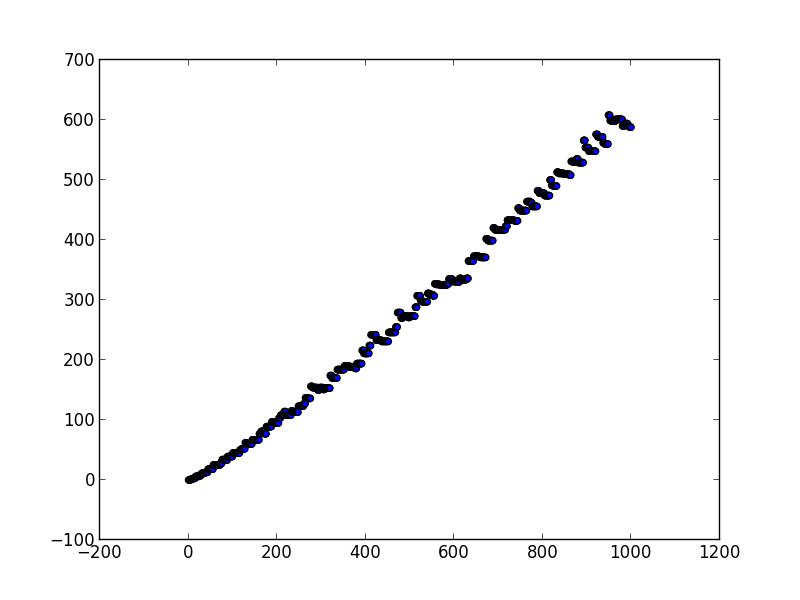
\includegraphics[width=0.4\linewidth]{TimeUntilStabilizeWithOnePeak}\label{fig:case1}} \qquad
%\subfigure[Horizontal axis is the number of chips on $(0,0)$ and vertical axis is the number of global earthquakes divided by the number of chips on $(0,0)$]{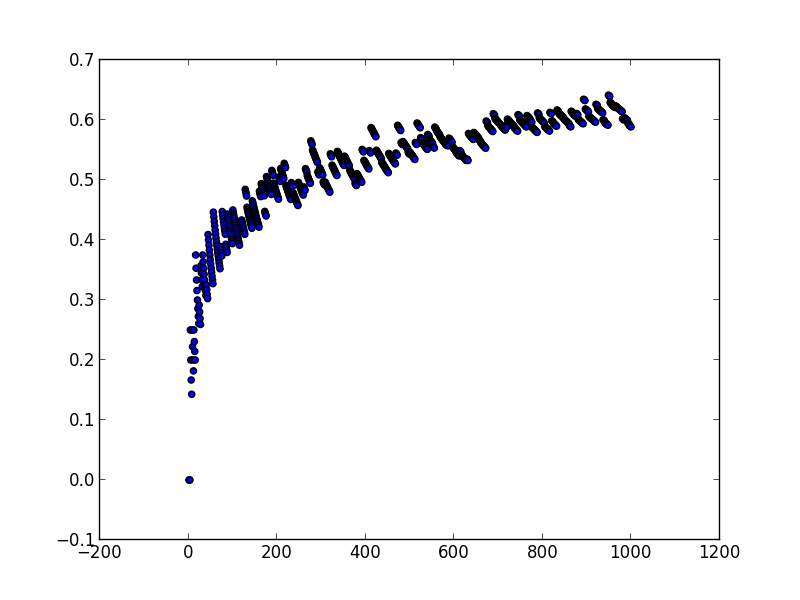
\includegraphics[width=0.4\linewidth]{Timeuntilstabledividedbyn}\label{fig:case2}}
%\caption{Number of global earthquakes until stability}
%\label{fig:growthofT}
%\end{figure}
%
%By looking at Figure~\ref{fig:growthofT} it seems that $T(n) = \Theta(n\log n)$. Our strategy to show a lower bound on $T(n)$ by giving a lower bound on $T'(0,0)$ seems to be the correct approach, since by experimental evidence (see Figure~\ref{fig:growthofT'}, we believe that $T'(0,0) = \Theta(n\log n)$.
%
%\begin{figure}[!ht]
%\centering
%\subfigure[Horizontal axis is the number of chips on (0,0) and vertical axis is the number of local earthquakes]{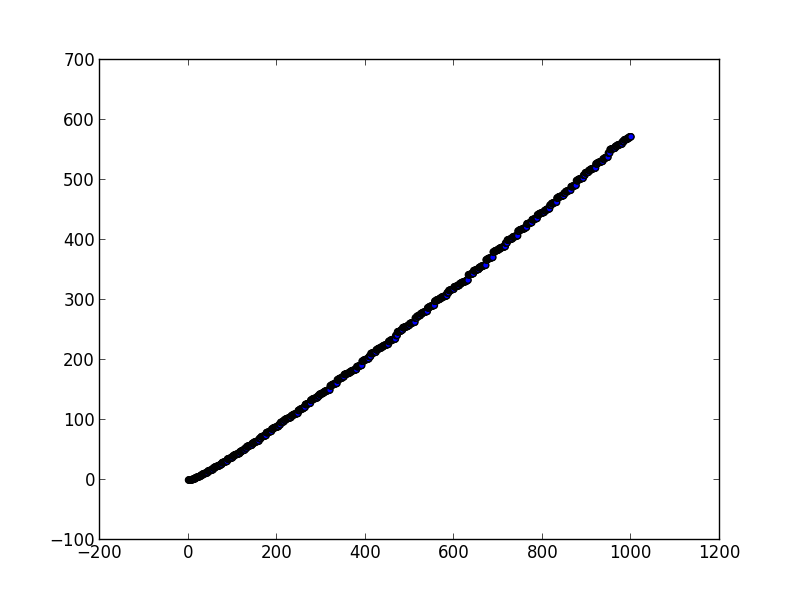
\includegraphics[width=0.4\linewidth]{centerearthquakes}\label{fig:case1}} \qquad
%\subfigure[Horizontal axis is the number of chips on (0,0) and vertical axis is the number of local earthquakes divided by the number of chips on (0,0).]{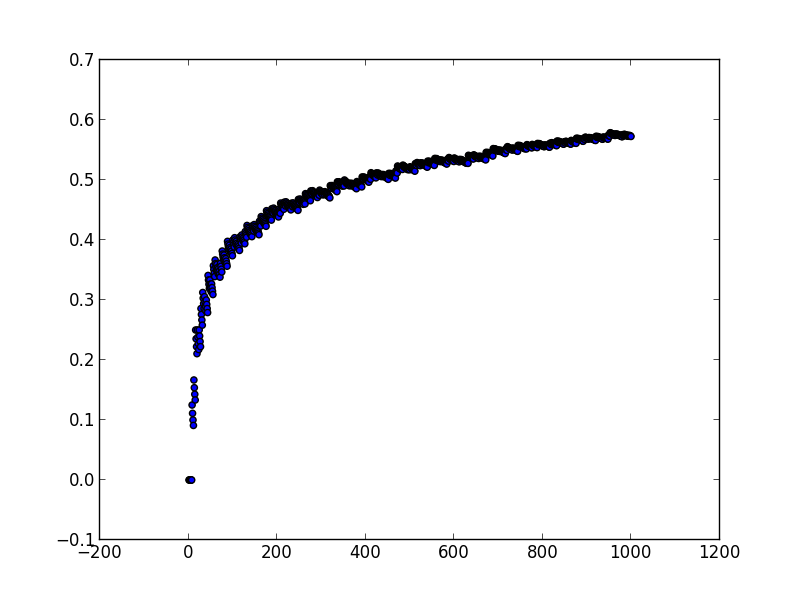
\includegraphics[width=0.4\linewidth]{centerearthquakesdividedbyn}\label{fig:case2}}
%\caption{Number of local earthquakes on (0,0) until stability}
%\label{fig:growthofT'}
%\end{figure}
%
%

\section{Board Variants: $d$-Trees}
\label{Board Variants: d-Trees}
\emph{written by Perry Kleinhenz, edited by Fermi Ma and Erik Waingarten.}\\

So far, we have analyzed the poker chips problem assuming that the underlying graph is an infinite grid graph. One important feature of this graph is that it is \emph{4-regular}, which means that each node has exactly 4 neighbors. Graphs where every node has an equal number of neighbors allow for an easy definition of the earthquake operation; if every node has $d$ neighbors, then an earthquake redistributes $d$ chips to each of the $d$ neighbors.

Thus, in this section we analyze how the problem changes when played over a large class of graphs that are regular, but are not grid-shaped.

\begin{definition}
A $d$-tree is a graph composed of a parent node connected by edges to $d-1$ unique children nodes.Those children each are connected by edges to $d-1$ unique children and so on.  
\end{definition}
\begin{figure}[!h]
\label{4tree}
\centering
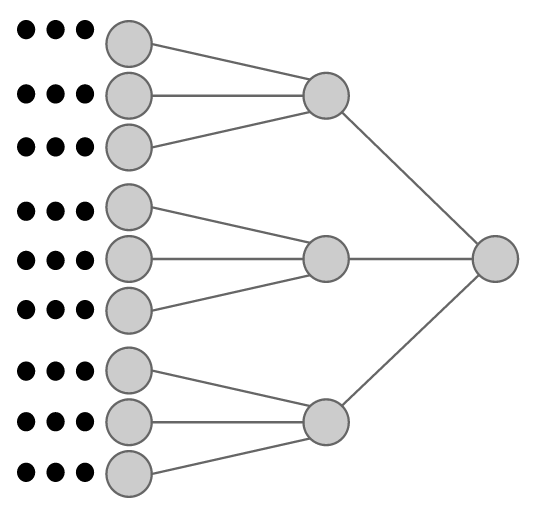
\includegraphics[width=0.4\linewidth]{4tree}
\caption{A 4-tree}
\end{figure}
We note that every node other than the original parent node has $d$ neighbors. In order to simplify our process we would like the graph to be regular and so we make the following definition. 
\begin{definition}
A joined $d$-tree is two $d$-trees connected at their parent nodes by an edge.
\end{definition}
\begin{figure}[!h]
\label{joined4tree}
\centering
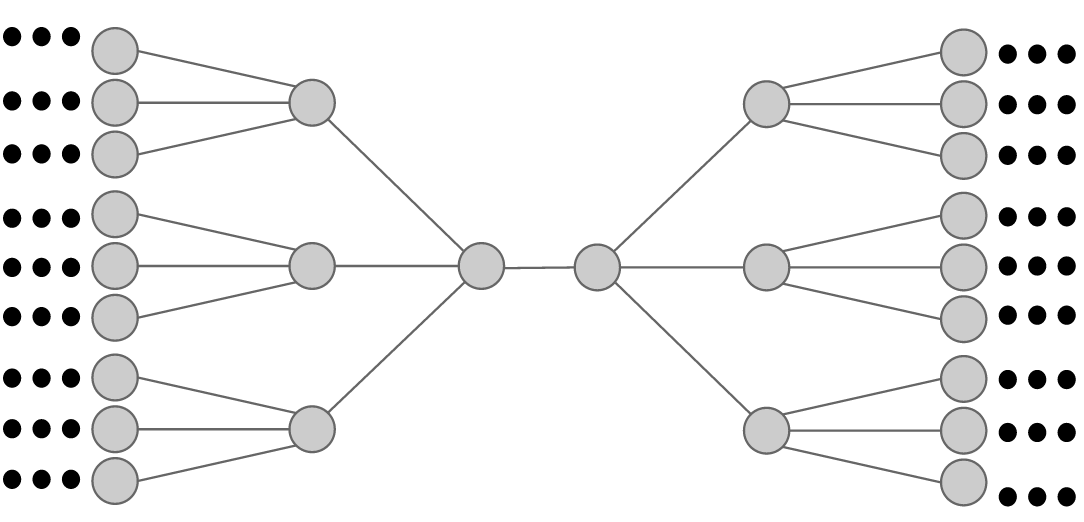
\includegraphics[width=0.8\linewidth]{joined4tree}
\caption{A joined 4-tree}
\end{figure}

We now define a coordinate system so that our method of proof can mirror that of the standard board case.
\begin{definition} We define a coordinate system for our joined $d$-trees, with the following rules:
\begin{enumerate}
	\item $(0,0)$ and $(1,0)$ are valid coordinates and refer to the two parent nodes.
	\item $(a,b)$ is a valid coordinate for $a<0$ if $0<b \leq (d-1)^{|a|}$
	\item $(a,b)$ is a valid coordinate for $a>1$ if $0<b \leq (d-1)^{|a-1|}$
\end{enumerate}
We define the set of all valid coordinates $G_d$ for a joined $d$-tree as 
\end{definition}
\begin{equation*}
G_d:= \{ (a,b) \in \mathbb{Z} \times \mathbb{Z} ; (a,b) \text{ obey the rules above}\}.
\end{equation*}


We now formalize the board of poker chips. Note that this definition only differs from our initial definition in that the input value is a coordinate of a node in a joined $d$-tree rather than a coordinate of the cartesian grid.
\begin{definition}
We define a $d$-board to be a function from the set of valid coordinates to the nonnegative integers, that is 
\begin{equation*}
b:  G_d \rightarrow \mathbb{Z}_{\geq 0}.
\end{equation*}
\end{definition}

In order to keep our notation compact we once again define a function that outputs the neighbors of a node
\begin{definition} 
Let $n(i,j)d$ be the set of neighbors of node $(i,j)$.
\end{definition}

We now define our earthquake operation in terms of $d$-boards. It functions analogously to the earthquake for the standard board, but instead of hitting nodes that have more than 4 chips it hits nodes that have more than $d$ chips. 
\begin{definition}
Let $E_s b$ be the board that results from an earthquake hitting the $d$-board $b$ at node $s$. If $b(s)>d$ then 
\begin{align*}
&E_s b(s) = b(s)- d \\
&E_s b(t) = b(t) +1 \quad \forall t \in n(s)
\end{align*}
Otherwise $b(s)<d$ the earthquake does not move any chips and $E_s b=b$.
\end{definition}

Now that we have formalized the earthquake operator we can introduce a precise definition of stability of a $d$-board. Noting that it is almost identical to definition of stability for a standard board. 
\begin{definition}
We say that a $d$-board is stable if its values are strictly less than $d$.
\end{definition}
This is equivalent to saying all earthquakes have no effect on the board. We also make a precise definition for a finite $d$-board.
\begin{definition} 
We say that a $d$-board is finite if the total number of chips on it is finite.
\end{definition}

We will now show that any finite $d$-board will stabilize after a finite number of earthquakes. Our method of proof will mirror the method used for the square lattice, without only minor changes.  Therefore we will introduce a new spread function that maps $d$-boards to positive numbers. We once again show that the spread function strictly increases after earthquakes are applied, which will imply that an earthquake irreversibly changes a board configuration. We will then give a bound on the maximum number of configurations a given $d$-board can be transformed into by earthquakes. Once again these together will show that all finite $d$-boards will stabilize.

We once again define a spread function 
\begin{definition}
$\Psi$ is a function from the finite $d$-boards and is defined as
\begin{equation*}
\Psi(b) = \sum_{(i,j) \in G_d} b(i,j) |i|^2.
\end{equation*}
Note that this is well defined for boards which contain a finite number of chips. 
\end{definition} 
We can once again think of this spread function as the sum of the number of chips on every node weighted by the taxi-cab distance from the node to the origin. 

We again demonstrate that nontrivial earthquakes increase the value of the spread function, using a nearly identical proof.
\begin{lemma} 
Suppose an earthquake hits node $s$ of a finite $d$-board $b$ producing the board $E_s b$. Then
\begin{equation*}
\Psi( E_s b) > \Psi (b).
\end{equation*}
\end{lemma}
\begin{proof}
Once again the chip stacks of the two boards are the same at all nodes except at $s$ and $n(s)$, the nodes that neighbor $s$. Thus the contribution to $\Psi$ is the same at all nodes except for those $d+1$.

If the first coordinate of $s$ is $s_1$ then the contribution to the spread function from node $s$ decreases from $b(s)|s_1|^2$ to $(b(s)-d)|s_1|^2$. 

Out of the $d$ nodes in $n(s)$ exactly $d-1$ of the neighbors of $s$ have a first coordinate with absolute value $||s_1| +1|$ and the remaining neighbor has a first coordinate with absolute value $||s_1| - 1|$ from the origin.  A point to emphasize is that this is the only substantial way in which this proof differs from the similar proof for the square lattice. 

We note that the contributions of these neighboring nodes increase by $||s_1| +1|$ and $||s_1|-1|$ respectively. 

Omitting the algebraic details we find that 
\begin{align*}
\Psi( E_s b) - \Psi(b) > d >0,
\end{align*}
which completes the proof.
\end{proof}


\begin{corollary}
\label{notreerepeats}
A finite $d$-board can never return to a previous state via a sequence of earthquakes
\end{corollary}
\begin{proof}
The proof is identical to that of Corollary ~\ref{norepeats}
\end{proof}

\begin{lemma}
\label{finiteextensiontree}
Suppose $\sum_{x,y} f(x,y) = C$, and the first coordinate of all nodes which are nonzero are in $[i_{min}, i_{max}]$. Then after applying any number of earthquakes the first coordinates of the nonzero nodes of the resultant board will be in range $[i_{min} - 2C, i_{max} + 2C]$.
\end{lemma}

\begin{proof}
It is obvious that a board with $C$ chips on nodes with first coordinate $l<0$ will have a lower $i_{min}$ than a board with $S$ chips on level 0, and the analogous statement for $i_{max}$ holds as well. 

Now because chips cannot be transferred between two nodes whose first coordinate differs by more than 1, we know that $C$ chips on a single node with first coordinate $l<0$ will have an $i_{min}$ no lower than $l-2C$ as there must be at least one chip on every other level. 

If we take any other arrangement of $C$ chips, with $i_{min}=l$ but not all $C$ chips are on a single node. We know that $i_{min}$ for this board is bounded below by $l-2C$. In order to have an $i_{min}$ below this at some point in time it would be possible to have $C$ chips on the same node on level $l$. But this cannot occur because in order to move a chip to a node with a lower first coordinate, one chip must moved to a node with a higher first coordinate. Therefore the resultant board does not have a node with a nonzero number of chips on it with first coordinate less than $i_{min} -2C$.

An analogous argument shows that  and after applying any sequences of earthquakes to $b$ the resultant board does not have a node with a nonzero number of chips on it with first coordinate greater than $i_{max}+2C$.
\end{proof}

\begin{theorem} If $b$ is a finite $d$-board then there exists some sequence $\{s_1, \ldots, s_k\}$ such that after applying an earthquake to each of these locations on $b$ the resultant $d$-board is stable.
\end{theorem}
\begin{proof}
The proof is identical to that of Theorem ~\ref{finitestability} with Lemma ~\ref{finiteextension} replaced by Lemma ~\ref{finiteextensiontree} and Corollary ~\ref{norepeats} replaced by ~\ref{notreerepeats}.
\end{proof}


\section{Computing with Chips}
\label{Computing with Chips}

\emph{Written by Erik Waingarten, edited by Fermi Ma and Perry Kleinhenz.}

In this section, we show how we can compute Boolean functions using the poker chip problem setup. In particular, we use the fact that Boolean functions can be represented as Boolean circuits, and we show how to construct elements of Boolean circuits using the poker chip board and earthquake operator.

We first introduce conventional definitions of Boolean variables and functions.
\begin{definition} 
A Boolean variable is a number in $\{0,1\}$, and a Boolean function is a function that takes in a finite number of Boolean variable and outputs a Boolean variable.
\end{definition}

We now introduce the standard Boolean functions. 
\begin{definition}
 The AND function takes in 2 Boolean inputs, and returns a 1 if and only if both the input values are 1. We will use $\vee$ to denote AND.
\end{definition}
\begin{definition}
The OR function, that takes in 2 Boolean inputs, and returns a 0 if and only if both input values are set to 0. We will use $\wedge$ to denote OR.
\end{definition}
\begin{definition}
The NOT function takes in 1 Boolean input; it returns a 1 if and only if the input value is a 0. We will use $\neg$ to denote NOT.
 \end{definition}
 If we think of associating 0 with ``false" and 1 with '``true", then the AND function returns ``true" if both inputs are ``true", and the OR function returns ``true" if at least one input is true. We can make more complicated Boolean functions with more than 2 inputs and compositions of these inputs. 
 
 We now begin to define Boolean circuits, first defining the two component parts, wires and gates.
\begin{definition}
 A wire is a device that in theory is capable of transmitting Boolean variables over arbitrarily long distances. If it takes in a 1 it will output a 1 and if it takes in a 0 it will output a 0. A gate is a boolean function that takes in an arbitrary number of wires and outputs an arbitrary number of wires.
\end{definition}
Examples of gates include AND gates and OR gates. In this section we will show that we can use the poker chips board to construct circuits that use AND and OR gates.

We now define a simple model of computation. We assume a finite board and specify some nodes as inputs nodes and some as outputs. If an input bit is to be set to 1, then we place 4 chips on the input node. Otherwise we do not place any chips on it. We then apply global earthquakes to the board until it stabilizes. If an output node ever has chips redistributed to it by an earthquake, then we set the output bit to 1; otherwise, the output bit is set to 0. 

A simple example of this is a board that computes the identity function of one input. We can compute 
\begin{equation*}
f(x) = x.
\end{equation*}
Our board has no chips on it, other than perhaps at the input node. We set the output node to be the same as the input node. If $x = 0$, then the input node does not have any chips on it and the board is stable. An earthquake never occurred on the output node and so the output is 0. If $x = 1$, then we place 4 chips on the input node and in order for the board to stabilize an earthquake must effect it. Because the input and output node are the same, this means an earthquake occurred on the output node and so the output is 1.


Using this simple model, there is a surprising number of things we can do. We can make wires, AND gates and OR gates (see Figure~\ref{fig:simplegates}). 

\begin{figure}
\centering
\subfigure[Wire]{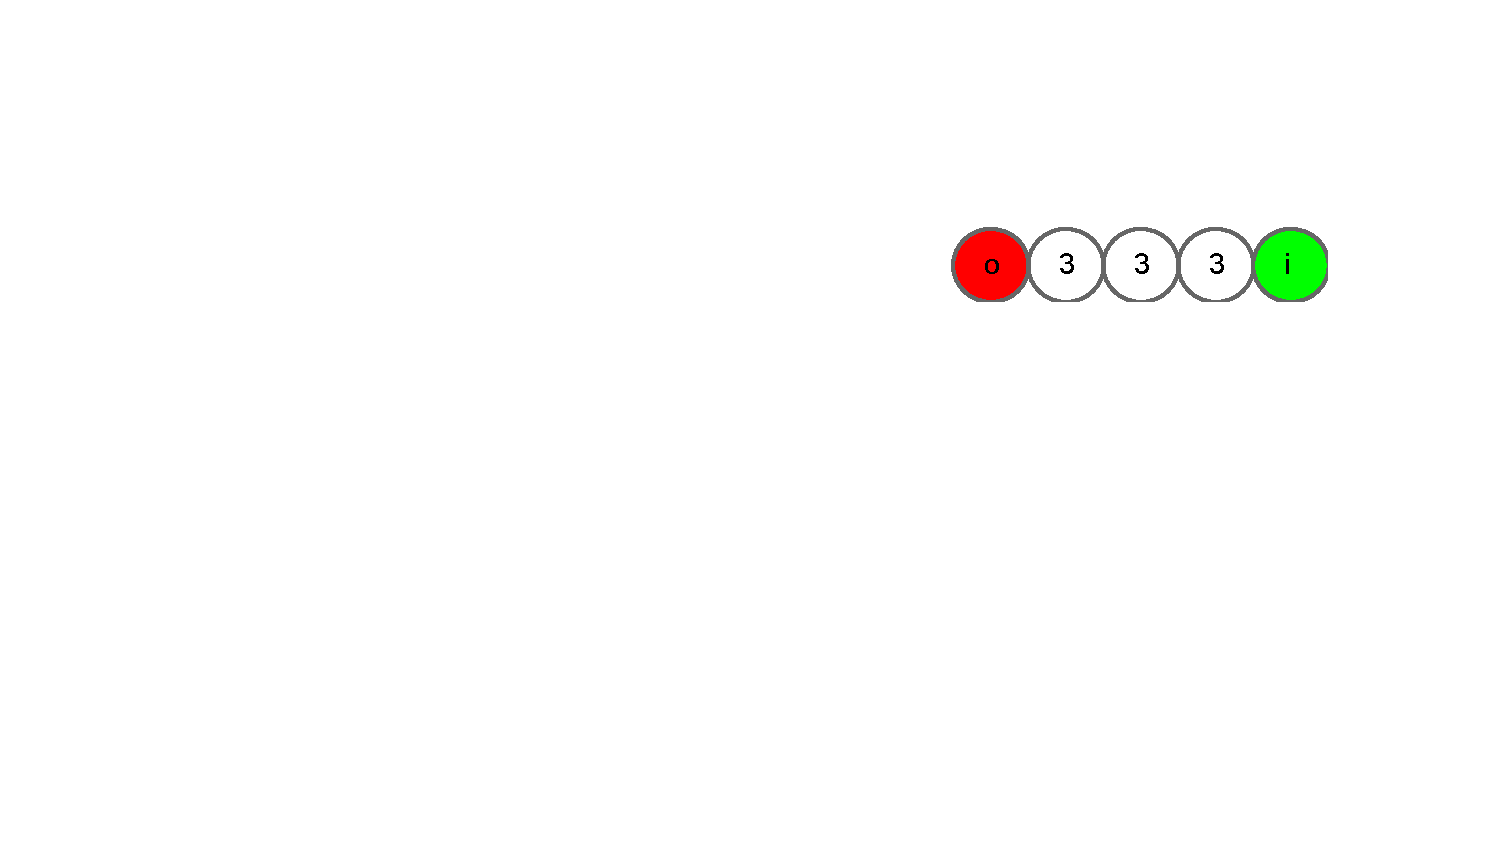
\includegraphics[width=0.25\linewidth]{wire.pdf}\label{fig:wire}}
\qquad\qquad
\subfigure[AND gate]{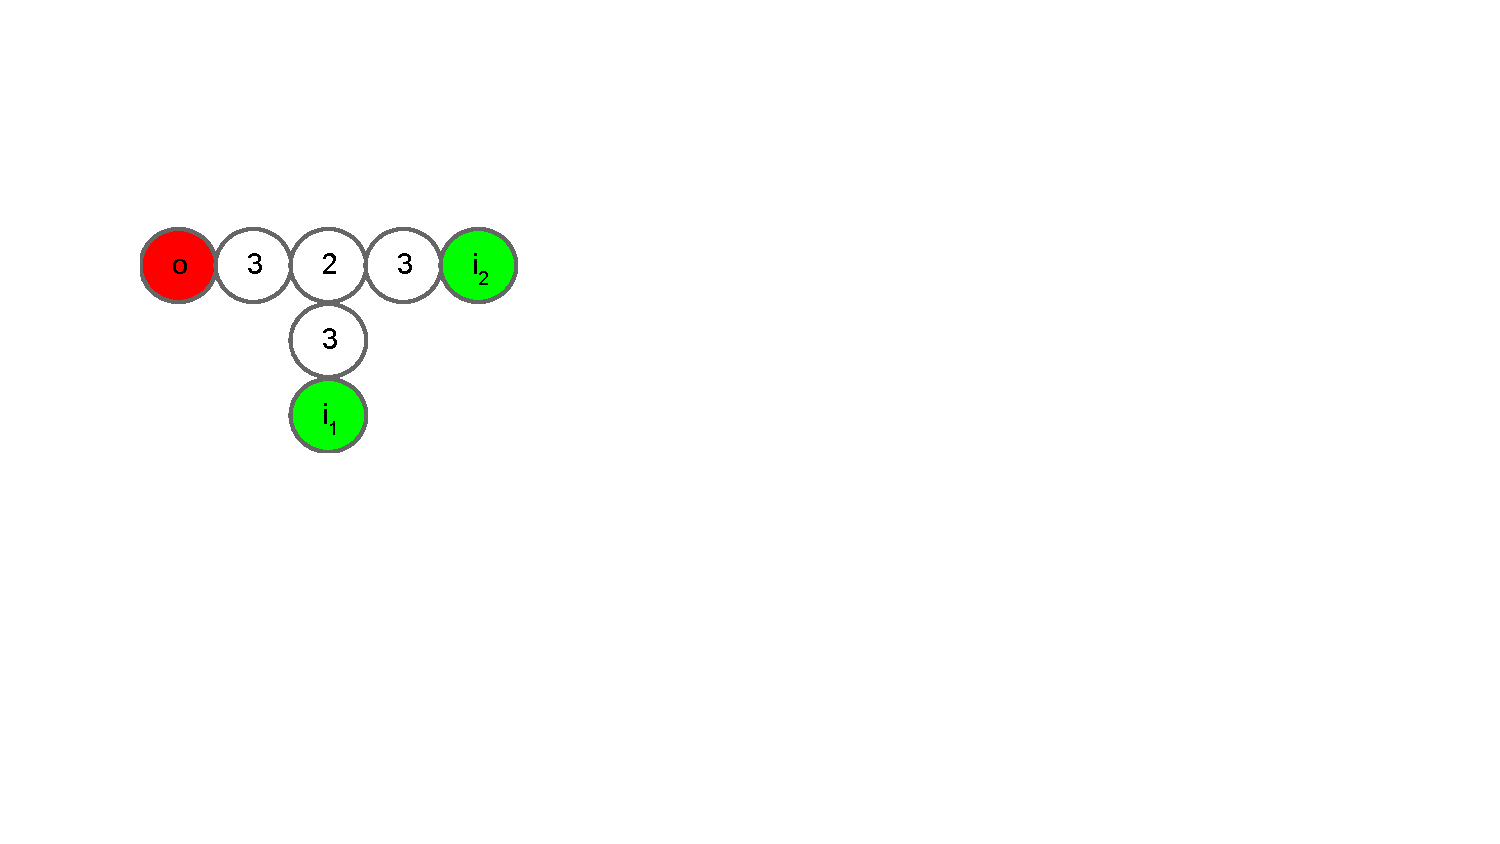
\includegraphics[width=0.25\linewidth]{andgate.pdf}\label{fig:AND}}
\qquad\qquad
\subfigure[OR gate]{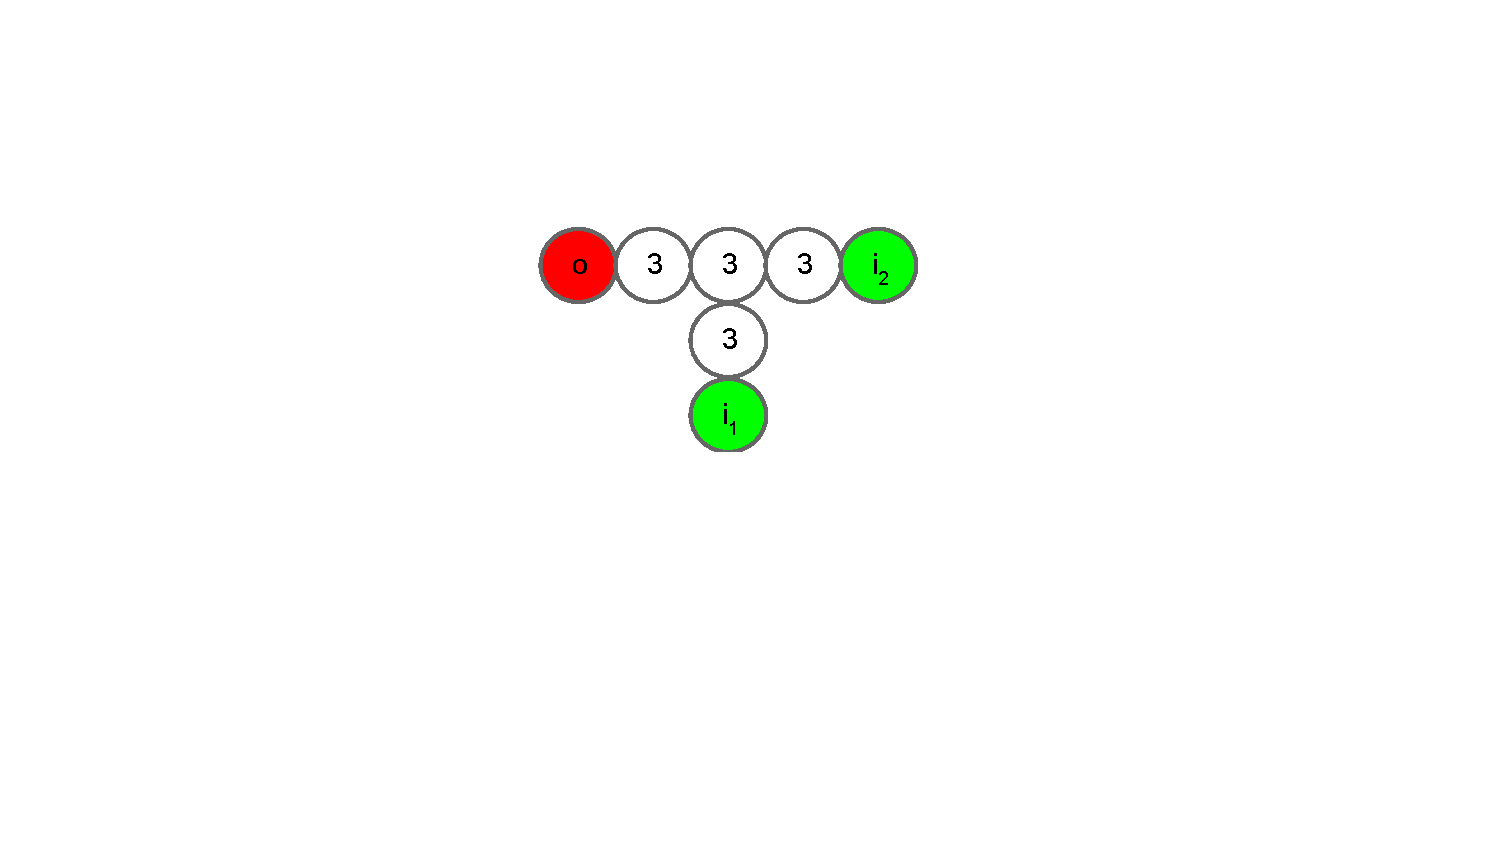
\includegraphics[width=0.25\linewidth]{orgate.pdf}\label{fig:OR}}
\caption{Gates in the simple model. Green are the inputs, red are the outputs. We disregard edges and assume that any two nodes that are touching have an edge between them.}
\label{fig:simplegates}
\end{figure}

Composing these gates, we can make circuits which can be used to compute certain Boolean functions. In particular we can compute any Boolean function that can be represented by a planar circuit composed of only AND and OR gates. However using this model we cannot construct a NOT gate.  

\begin{theorem}
There does not exist a board which computes $f(x) = \neg x$.
\end{theorem}

\begin{proof}
Suppose for contradiction that we have a board with one input $i$ and one output $o$ which computes NOT.  Then we know that there exists some node which initially has over $4$ chips otherwise the board would be stable and the output could never be effected by an earthquake. 

Let $A(0)$ be the set of nodes that are targeted by earthquakes when $i = 0$ and $A(1)$ be the set of nodes that are targeted by earthquakes when $i=1$.  We claim that $A(0) \subset A(1)$. This is true as when we set the input square to 1, we only increase the locations that can have chips redistributed to them by earthquakes. However the output square is not in $A(1)$ by the definition of our function, which produces a contradiction. Therefore our current model of computation cannot have a board that computes NOT. 
\end{proof}

%\begin{lemma}
%Let $A(i)$ be the set of active nodes in an execution of board $b$ with input node $i$. Then $A(0) \subset A(1)$.
%\end{lemma}

%\begin{proof}
%By Theorem~\ref{thm:order}, we can simulate an execution of the board with input be 0 before we apply earthquakes to the input node. We start with a board $b$ where the input is 1, so it has 4 chips. We simulate by applying earthquakes to the active nodes that are not the input. If the input node ever receives more than $8$ chips, we apply one earthquake to the input node. This way, we guarantee that the input node always contains more than $4$ chips. In addition, the input node does not contain more than $7$ chips for more than one consecutive earthquake.
%We do this until every node except the input node has less than 4 chips.

%Note that this execution is indistinguishable from the execution with input set to 0. This means that all nodes activated in the execution with input 0 are the same as the nodes activated in the above mentioned execution. 

%Once this is done, then we continue with the execution applying the earthquake to the input node. By Theorem~\ref{thm:order}, the final configuration will be the same as any execution of the board. So $A(0) \subset A(1)$.
%\end{proof}

We now introduce a slightly more complicated model for computation that will allow us to build NOT gates as well as AND and OR gates. As before, we assume a finite board with finitely many chips. We again specify certain nodes as inputs and outputs, placing 4 chips on input bits that are to be set to 1. We also designate a specific node $r$ that can be any node including inputs and outputs. When $r$ is affected by an earthquake, we finish redistributing all of the chips and read the outputs, setting an output to be 1 if it has 4 chips on it and 0 otherwise. 

We show how to make a board that computes the identity, as well as AND and OR gates. They are essentially the same as in our simpler model of computation but they include now include an $r$ node.

\begin{figure}
\centering
\subfigure[Wire]{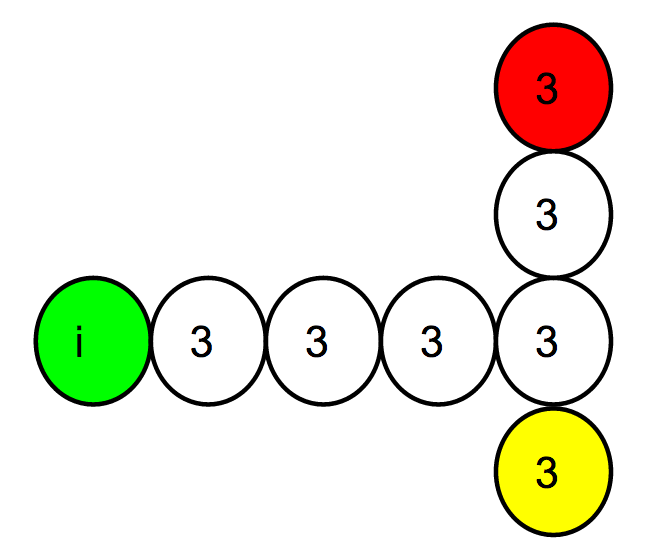
\includegraphics[width=0.25\linewidth]{wirewithr}\label{fig:wirer}}
\qquad\qquad
\subfigure[AND gate]{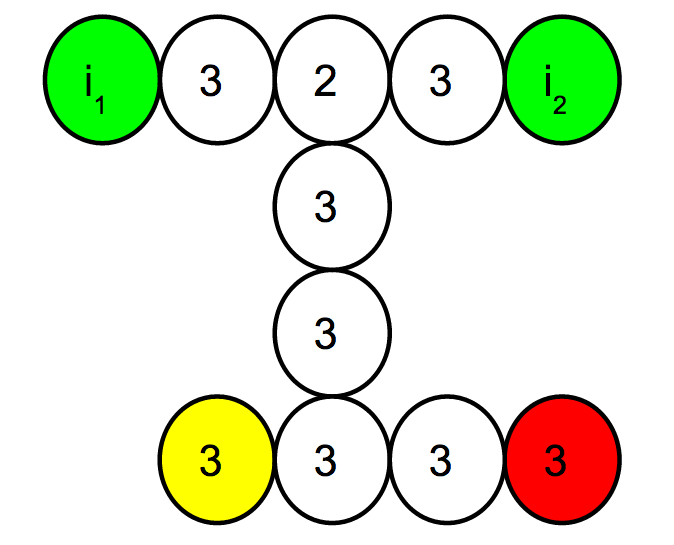
\includegraphics[width=0.25\linewidth]{andwithr}\label{fig:ANDr}}
\qquad\qquad
\subfigure[OR gate]{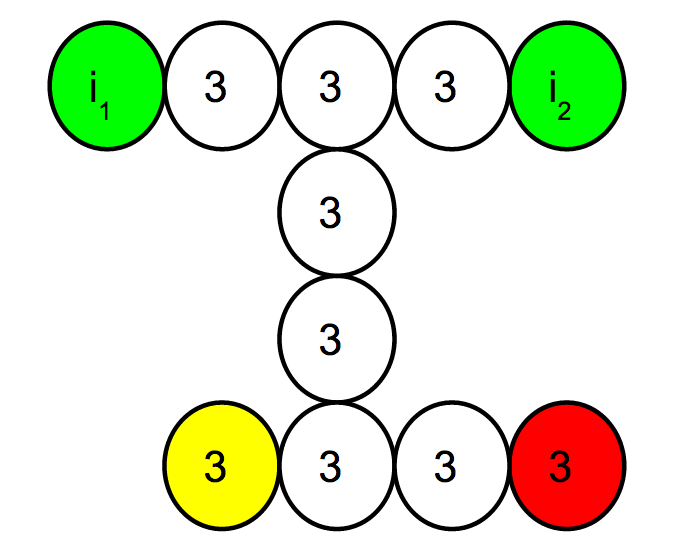
\includegraphics[width=0.25\linewidth]{orwithr}\label{fig:ORr}}
\caption{Gates in the our more complicated model. Green are the inputs, red are the outputs and yellow is the node $r$. We disregard edges and assume that any two nodes that are touching have an edge between them.}
\label{fig:simplegateswithr}
\end{figure}


%Turning is non trivial, we must guarantee that we can turn a signal and align the timinings of the inputs and outputs in the clock so that they have the same distance. this is a counter-clockwise turn where $c$ denotes the clock, $i$ is the input bit, then $r$ is the output read and $o$ is the output bit.


%Since the clock snakes along the path while $i$ takes the shorter path. 
%Likewise, we can perform a clockwise path by making $i$ snakes while the clock takes a straight path. 

%We can synchronize the input so that the input signal waits for the clock to arrive. This can be simply done with the following board configuration:

%Note that the path from $i$ to $o$ is 6 units long, while the path from clock is 12 unit long. $i$ waits for the clock since it needs the signal from $c$ from two sides to activate the 1 in the path from $i$ to $o$.

%The fact that we have a synchronizer means that the model of computation is equivalent to one where there is only one clock for all input bits. 

%Now we can show how to compute some basic boolean functions and since we have turns and synchronizers, we can assume that we have synchronized the inputs already. The following can compute the AND of two inputs. 

%Where we can make the $c_1$ and $c_2$ snake around before hand to guarantee that they are synchronized, and then we can make $c_1$ snake around so that it becomes the clock of the output. So in this case, $o = i_1$ AND $i_2$.

%Similarly, we can compute the OR of two circuits with a very simple modification:
%And we can do a similar set up to synchronize the clocks. 

Our goal in introducing this more complicated model of computation is to allow ourselves to build a board that can compute NOT. The following board does so:
\begin{figure}
\centering
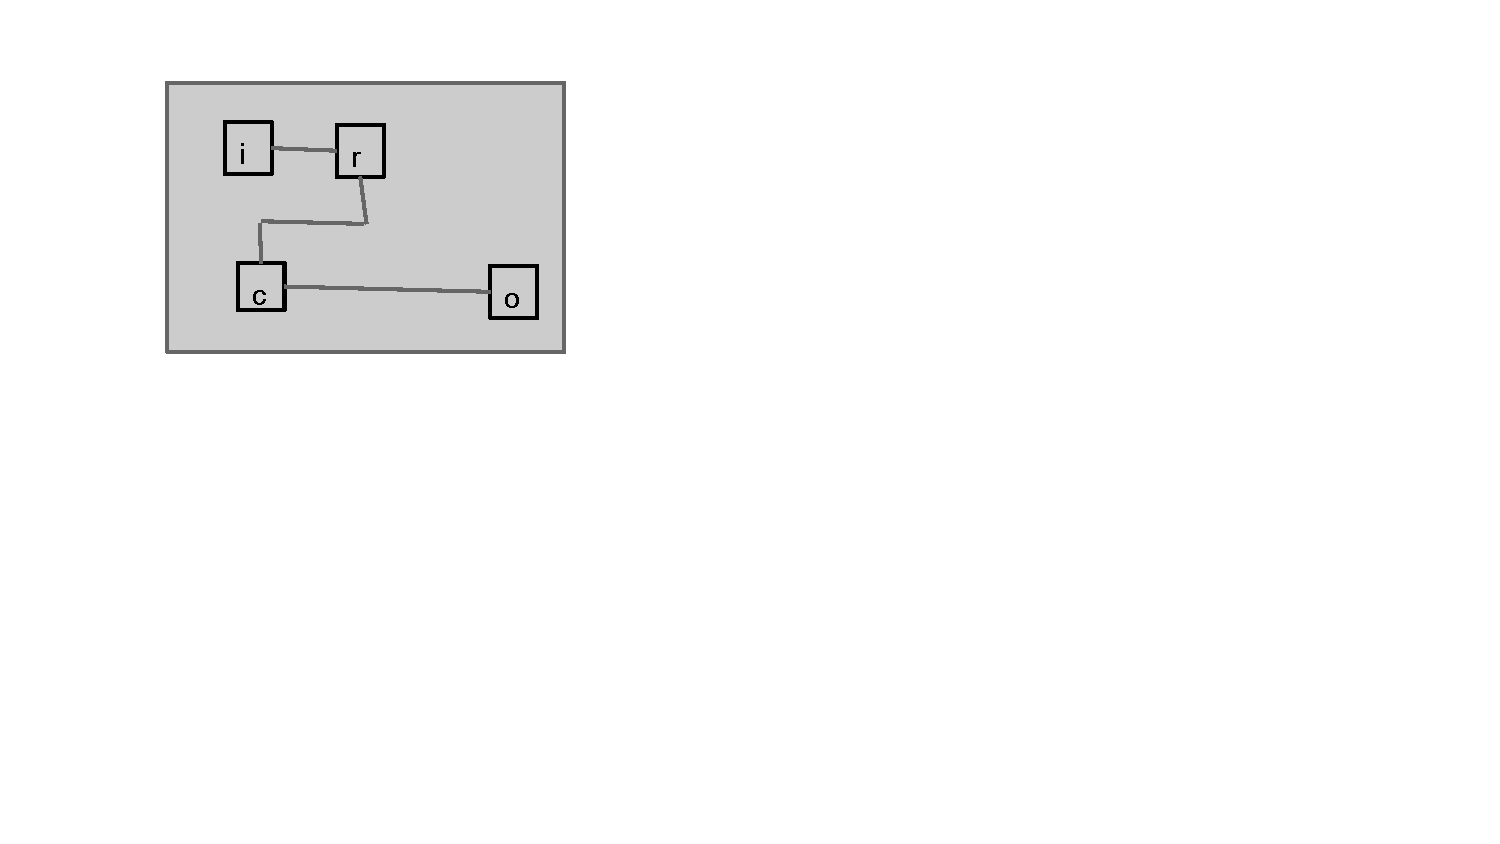
\includegraphics[width=0.5\linewidth]{notgate}
\caption{Board which computes $f(x) = \neg x$}
\label{fig:NOT}
\end{figure}

We note that in Figure~\ref{fig:NOT}, the number of nodes between the 4 and $r$ is same as the number of nodes between the 4 and the output node, but the number of nodes separating the input node and $r$ is shorter than the number of nodes separating the 4 and the output node. If $i$ is set to $1$, then $r$ will be activated while the output only has 3 chips on it, so the output will be read as 0. If the input is set to 0, then $r$ and the square adjacent to $o$ will both have 4 chips on them at same time so the output will be $1$. This computes $f(x) = \neg x$. However, we have switched the standard positions of $r$ and the output node, so it is unclear how to compose this board with other ones. 

\section{Three Haikus}

Poker board with chips\\
Suddenly hit by earthquakes.\\
Can never return. \\

\noindent Another earthquake\\
hits the board, and then one more.\\
Who cares which was first! \\ 

\noindent Now the aftershock\\
is computing some functions\\
---but just basic ones!
\end{document}
